%% -*- coding: utf-8 -*-

\documentclass[12pt,a4paper]{report}
\usepackage[left=2cm,right=2cm,
    top=2cm,bottom=2cm,bindingoffset=0cm]{geometry} 
\usepackage[utf8]{inputenc}
\usepackage[english,russian]{babel}
\usepackage{indentfirst}
\usepackage{misccorr}
\usepackage{graphicx}
\usepackage{amsmath}
\usepackage{amsfonts}
\usepackage{amssymb}
\setcounter{page}{2}

\begin{document}
\begin{titlepage}
\newpage
  \begin{center}
     
    Санкт-Петербургский Политехнический Университет Петра Великого \\
    
    Институт компьютерных наук и технологий \\
    
    Кафедра компьютерных систем и программных технологий
    \end{center}
    
    \vspace{15em}
    \begin{center}
    \textsc{Лабораторная работа №1}\\
    \vspace{5mm}
    \textsc{Сигналы телекоммуникационных\\
      систем}
    
   \end{center}
\vspace{10em}

\newlength{\ML}
\settowidth{\ML}{«\underline{\hspace{0.7cm}}» \underline{\hspace{2cm}}}
\hfill\begin{minipage}{0.45\textwidth}
\vfill
  Руководитель \\
  \\
  \underline{\hspace{\ML}} Богач Н.\,В.\\
 
\end{minipage}%
\bigskip

\hfill\begin{minipage}{0.45\textwidth}
  Выполнил\\
  \\
  \underline{\hspace{\ML}} Солдатова Е.\,И.\\
  группа 33501/3
\end{minipage}%

\vspace{\fill}
\begin{center}
    
  Санкт-Петербург\\
   2018 
\end{center}
\end{titlepage}

\paragraph{1. Цель работы\\\\}
Познакомиться со средствами генерации сигналов и визуализации их спектров.

\paragraph{2. Постановка задачи\\\\}
В командном окне MATLAB и в среде Simulink промоделировать синусоидальный и прямоугольный сигналы с различными параметрами. Получить их спектры. Вывести на график.
\paragraph{3. Теоретическая часть\\\\}
В состав системы MATLAB входит пакет моделирования динамических систем – Simulink. Пакет Simulink позволяет осуществлять моделирование и исследование поведения динамических нелинейных систем. Ввод характеристик исследуемых систем производится в диалоговом режиме, путем графической сборки схемы соединений элементарных стандартных звеньев. В результате такой сборки образуется модель исследуемой системы. Модель хранится в файле с расширением .mdl.
Процесс построения модели Simulink включает в себя компоновку и задание необходимых параметров. Компоновка заключается в выборе из библиотекSimulink необходимых блоков, размещение их в открывшемся окне и задание межблочных связей. Далее для каждого блока устанавливаются соответствующие параметры, отвечающие требованиям моделируемой системы.

Сигналом называется физический процесс или явление, несущее сообщение о каком-либо событии, состоянии объекта, либо передающее команды управления, оповещения и т.д. Таким образом, сигнал является материальным носителем сообщения. Таким носителем может служить любой физический процесс (свет, электрическое поле, звуковые колебания и т.п.). В данной работе мы будем рассматривать синусоидальные (гармонические) и прямоугольные (негармонические) сигналы.

Существует общая методика исследования периодических негармонических сигналов в электрической цепи, которая основана на разложении сигналов в ряд Фурье. Данная методика состоит в том, что всегда можно подобрать ряд гармонических сигналов с такими амплитудами, частотами и начальными фазами, алгебраическая сумма ординат которых в любой момент времени равна ординате исследуемого несинусоидального сигнала. Совокупность гармонических составляющих, образующих сигнал несинусоидальной формы, называется спектром этого негармонического сигнала.

Всякая периодическая функция $y(t)$, удовлетворяющая условиям Дирихле, может быть представлена в виде ряда Фурье:
  \begin{center}
		$y(t) = \sum_{k=-\infty}^{\infty}C_ke^{j2{\pi}ft}$ \\
  \end{center}
где $f=\frac{1}{T}$;$T$ --- период функции $y(t)$; $C_k$ --- постоянные коэффициенты.
В качестве базовых функций использованы комплексные гармонические функции вида $e^{j2{\pi}ft}$, где $k$ --- целочисленный параметр. Значения коэффициентов $C_k$ можно определить по формуле:\\\\
  \begin{center}
		$C_k = \frac{1}{T}\int_{t_0}^{t_0+T}y(t)e^{-j2{\pi}kft}dt$\\
  \end{center}
Ряд Фурье справедлив для периодических сигналов. Для непериодических сигналов используется интеграл Фурье:
  \begin{center}
${\phi}(t)=\int_{-\infty}^{\infty}{[\int_{-\infty}^{\infty}{{\phi}(t)e^{-j2{\pi}ft}dt}]e^{j2{\pi}ft}df}$
  \end{center}


\paragraph{4. Ход работы\\\\}
\textbf{Построение синусоидального сигнала и его спектра в командном окне Matlab:\\}

Текст программы:\\
\\
ts=0.01 \% задаем частоту дискретизации\\
t = 0:ts:2*pi; \\
N = 256;\\
f0 = 5;\\
\% исходный сигнал\\
y = sin(2*f0*pi*t);\\
plot(t(1:200),y(1:200)) \\
grid\\
\% спектр исходного сигнала\\
figure\\
\% прямое преобразование Фурье\\
plot(abs(fft(y, N)))\\

Результат работы программы - на рис.1 и 2\\
\begin{figure}[h!]
\center{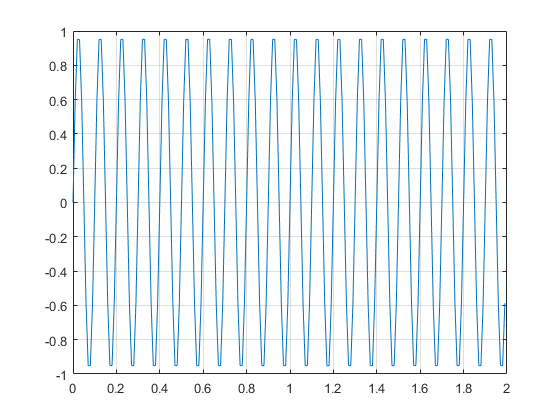
\includegraphics[width=0.6\linewidth]{Sin_signal}}
\caption{Синусоидальный сигнал.}
\end{figure}
\begin{figure}[h!]
\center{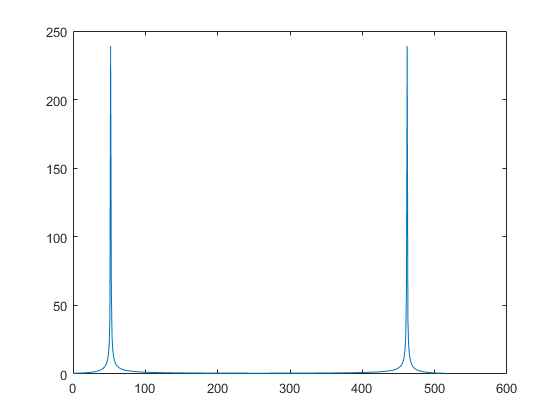
\includegraphics[width=0.6\linewidth]{Sin_spectr}}
\caption{Спектр синусоидального сигнала.}
\end{figure}
\newpage
\textbf{Построение прямоугольного сигнала и его спектра в командном окне Matlab:\\}

Текст программы:\\
\\
tau=5*10\^(-3); \\
q = 5; \% скважность\\
n=1024;\\
Tp=tau*q;\\
N=4;\% число импульсов\\
T=N*q*tay; \\
Ts=T/(n-1);\\
d=(0:N-1)*Tp;\% вектор задержки \\
t=0:Ts:T; \\
A=5;\\
fd=(64*(2/q))/(q*tay);\\
\% исходная последовательность импульсов\\
s=A*pulstran(t,d,'rectpuls', tay);\\
figure;\\
plot(t,s);\\
x=A*rectpuls(t,tay);\\
x=A*2*x/(q*sum(x));\\
f=0:fd/n:fd/2-1/n;\\
X=fft(x,n);\\
Z=abs(X);\\
figure;\\
plot(f,Z(1:length(f))), xlim([0 3/(q*tay)])\\
\\
Результат работы программы - на рис.3 и 4\\
\newpage
\begin{figure}[h!]
\center{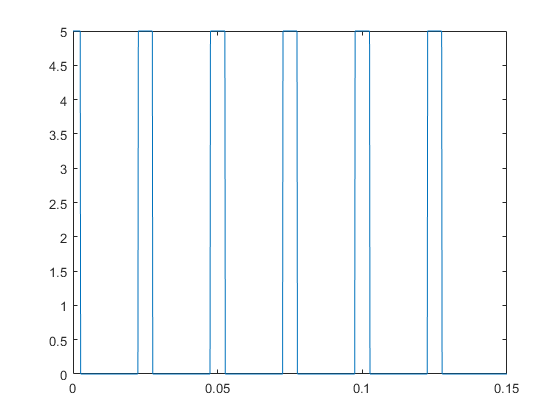
\includegraphics[width=0.6\linewidth]{Rect_signal}}
\caption{Прямоугольный сигнал.}
\end{figure}
\begin{figure}[h!]
\center{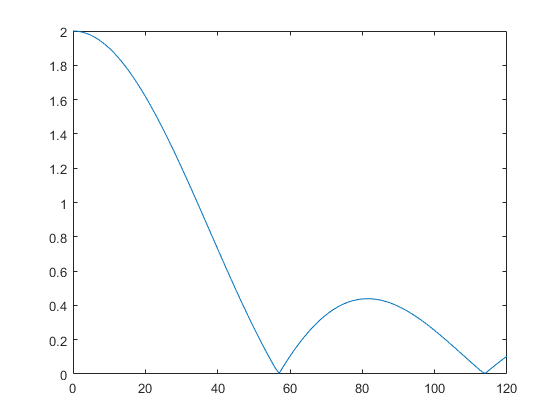
\includegraphics[width=0.6\linewidth]{Rect_spectr}}
\caption{Спектр прямоугольного сигнала.}
\end{figure}
\newpage
\textbf{Построение синусоидального сигнала и его спектра в среде Simulink:\\\\}
Схема построения в среде Simulink - на рис.5.
\begin{figure}[h!]
\center{\includegraphics[width=0.6\linewidth]{Sin_sim}}
\caption{Схема построения синусоидального сигнала.}
\end{figure}

Результаты работы - на рис. 6 и 7.
\begin{figure}[h!]
\center{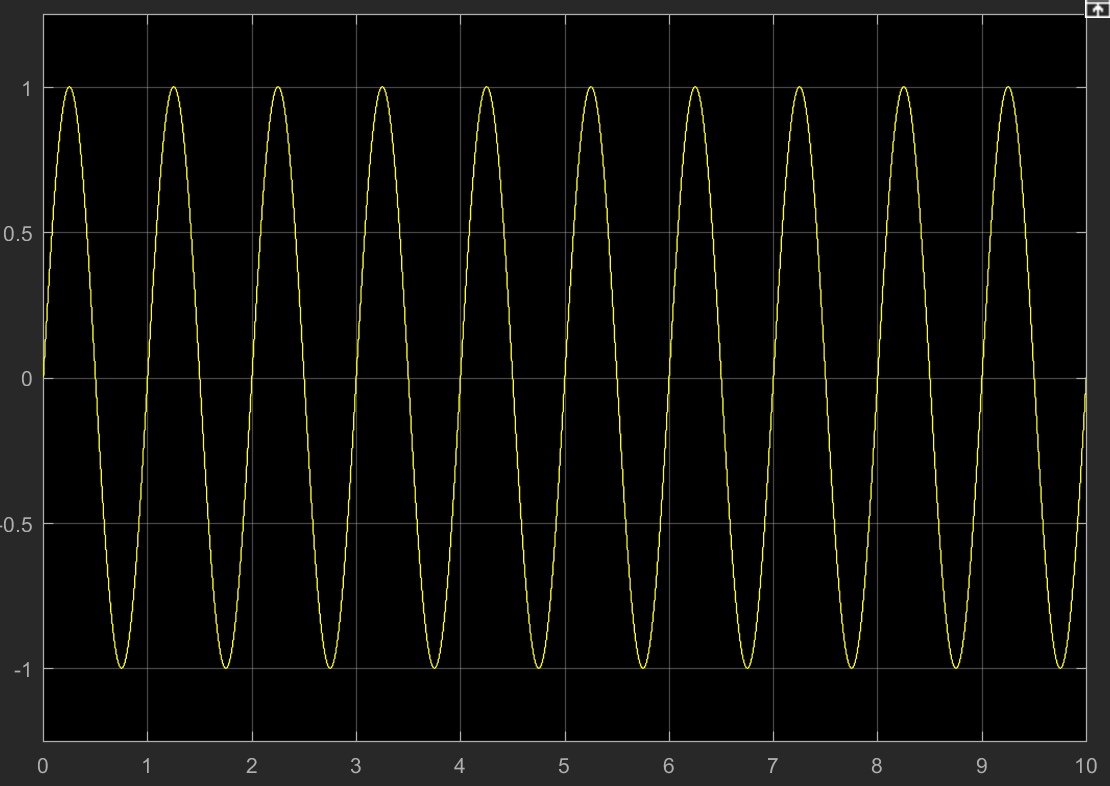
\includegraphics[width=0.6\linewidth]{Sin_signal_sim}}
\caption{Синусоидальный сигнал.}
\end{figure}
\begin{figure}[h!]
\center{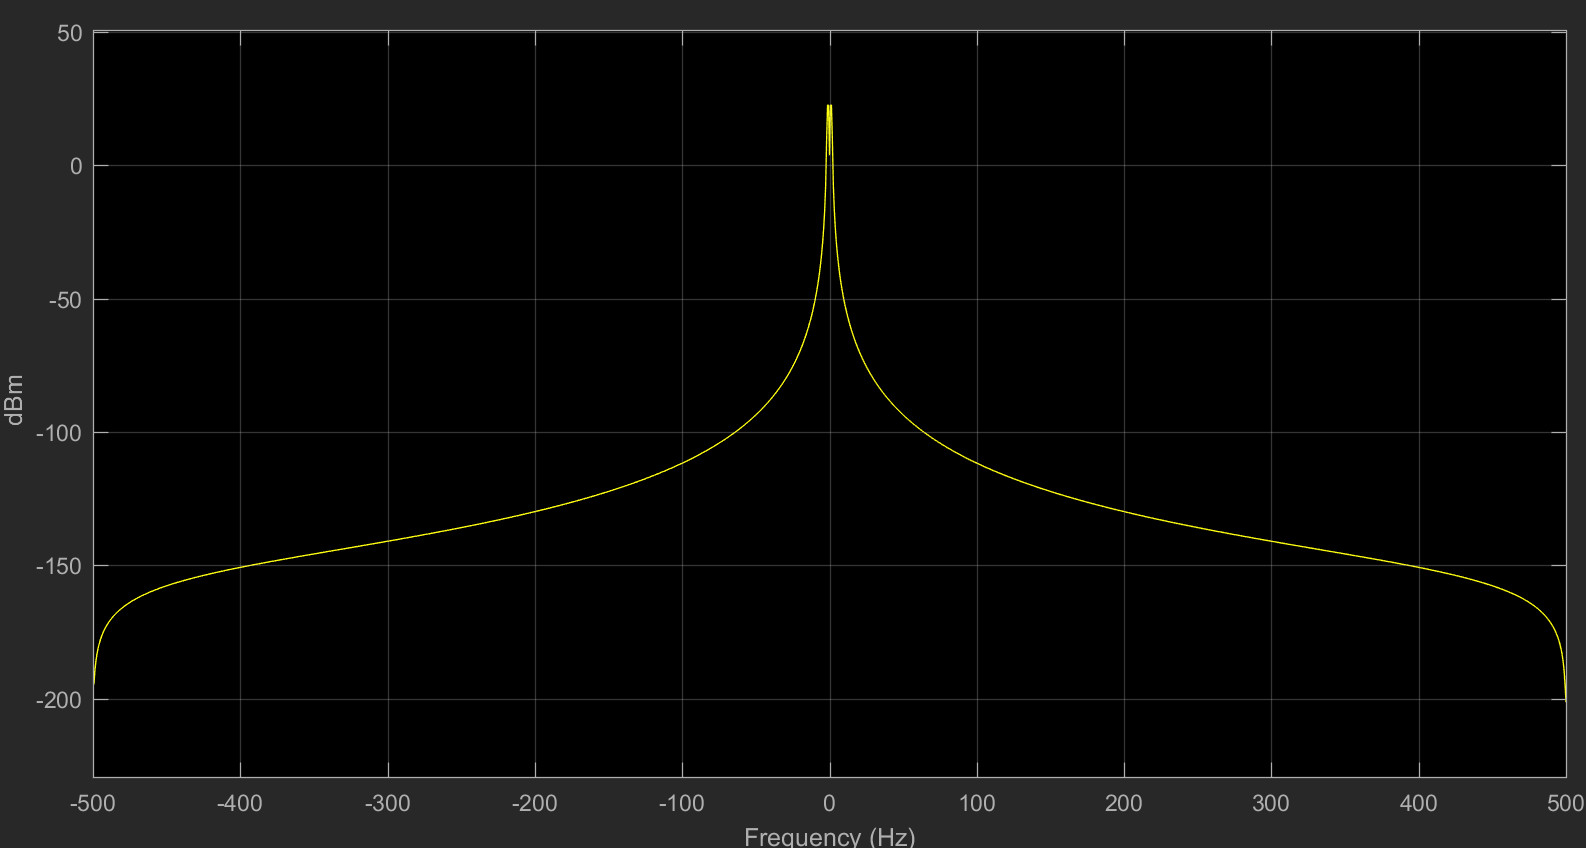
\includegraphics[width=0.6\linewidth]{Sin_spectr_sim}}
\caption{Спектр синусоидального сигнала.}
\end{figure}
\newpage
\textbf{Построение прямоугольного сигнала и его спектра в среде Simulink:\\\\}
Схема построения в среде Simulink - на рис.8.
\begin{figure}[h!]
\center{\includegraphics[width=0.6\linewidth]{Rect_sim}}
\caption{Схема построения прямоугольного сигнала.}
\end{figure}

Результаты работы - на рис.9 и 10
\begin{figure}[h!]
\center{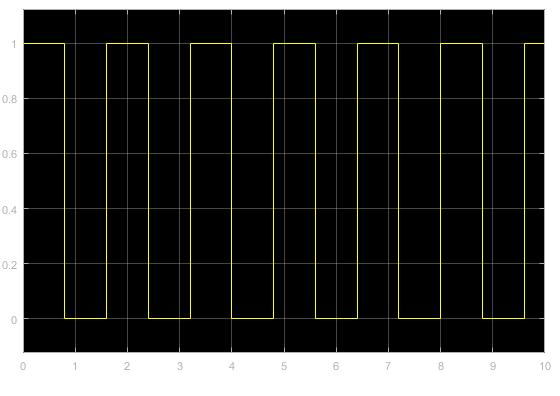
\includegraphics[width=0.6\linewidth]{Rect_signal_sim}}
\caption{Прямоугольный сигнал.}
\end{figure}
\begin{figure}[h!]
\center{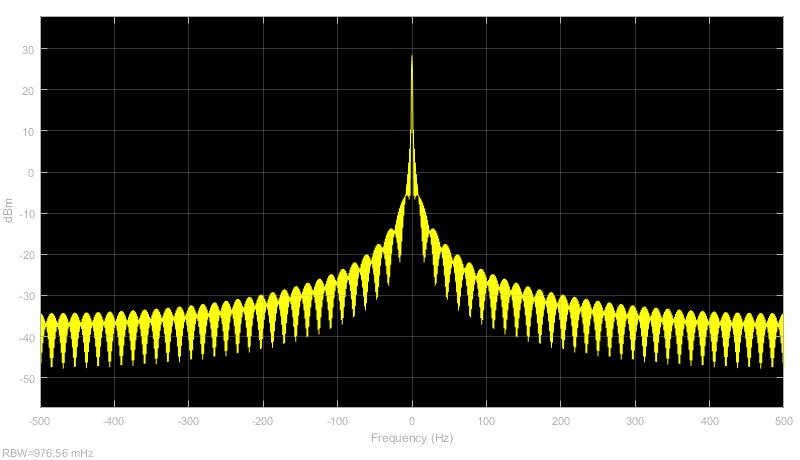
\includegraphics[width=0.6\linewidth]{Rect_spectr_sim}}
\caption{Спектр прямоугольного сигнала.}
\end{figure}
\newpage
\paragraph{5. Выводы\\\\}
В командном окне MATLAB и в среде Simulink
были промоделированы синусоидальный и прямоугольный сигналы. Были получены их спектры.

как получить спектр какие бывают сигналы (конечные бесконечные) у какого сигнала какой спектр

Любой сигнал описывается набором параметров, являющихся его признаками. Рассмотрим параметры изученных сигналов.

Информационными параметрами гармонического сигнала являются амплитуда сигнала, фаза, период.

Информационными параметрами прямоугольного сигнала яляются период повторения импульсов, длительность импульсов, скважность импульсов (отношение периода к длительности.
\end{document}
